\documentclass[a4paper, c]{beamer}

\usepackage[utf8]{inputenc}
\usepackage[french]{babel}

\usepackage{amsmath}
\usepackage{amsfonts}

\DeclareMathOperator*{\argmin}{arg\,min}

\usetheme{Boadilla}
\setbeamertemplate{navigation symbols}{}

\title{Optimisation distribu\'ee}

\begin{document}

\section{Rappel du problème}

\begin{frame}
    \frametitle{Modèle}

    \begin{columns}
        \begin{column}{.5\textwidth}
            \begin{itemize}
                \item $G = (V, E)$
                \item $V = \{1,\ldots,n\}$
                \item Caractéristiques : $(X_i)_{1\leq i \leq n}$
            \end{itemize}
        \end{column}
        \begin{column}{.3\textwidth}
            \begin{center}
                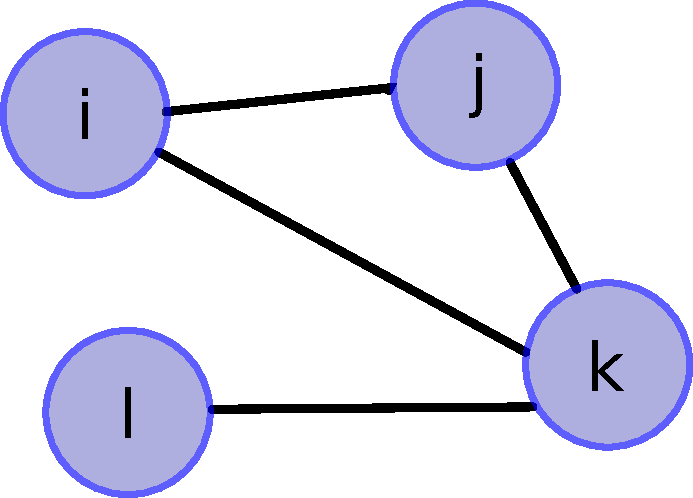
\includegraphics[width=.9\textwidth]{Figures/graph.pdf}
            \end{center}
        \end{column}
    \end{columns}
    \vspace{.5cm}
    Objectif : regrouper par similarité suivant les caractéristiques
\end{frame}

\begin{frame}
    \frametitle{Formulation du problème}

    \begin{itemize}
        \item Problème :
        \[
            \min_{P \in \mathcal{P}} w(P) = \frac{1}{n^2} \sum_{1 \leq i,j \leq n} D(X_i, X_j) \Phi_P(X_i, X_j)
        \]
    \begin{itemize}
        \item $D$ : mesure de dissimilarit\'e
        \item $\mathcal{P}$ : ensemble des partitions admissibles
        \item $\Phi_P$ : indicatrice de \emph{cluster}
    \end{itemize}

    \item Contraintes suppl\'ementaires :
    \begin{itemize}
        \item Distribution du calcul
        \item Certains $D(X_i, X_j)$ sont inaccessibles
    \end{itemize}
    \end{itemize}

\end{frame}

\section{Optimisation distribu\'ee}

\begin{frame}
    \frametitle{Principe des algorithmes de \emph{gossip}}

    \begin{columns}
        \begin{column}{.6\textwidth}
            Le n\oe{}ud $i$ :
            \begin{itemize}
                \item dispose de l'information $A_i$
                \item effectue une estimation $P_i$
                \item<2-> reçoit les estimations de ses voisins
                \item<4-> transmet son estimation à ses voisins
            \end{itemize}
        \end{column}
        \begin{column}{.4\textwidth}
            \only<1>{
                \begin{center}
                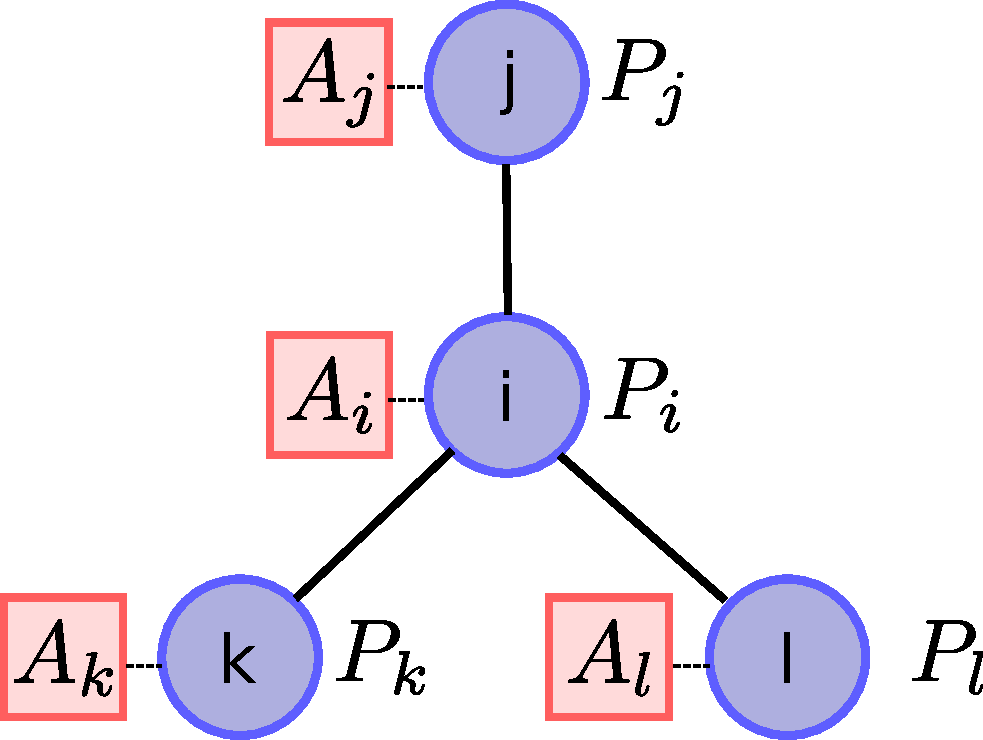
\includegraphics[width=.9\textwidth]{./Figures/gossip_1.pdf}
            \end{center}
            }
            \only<2>{
                \begin{center}
                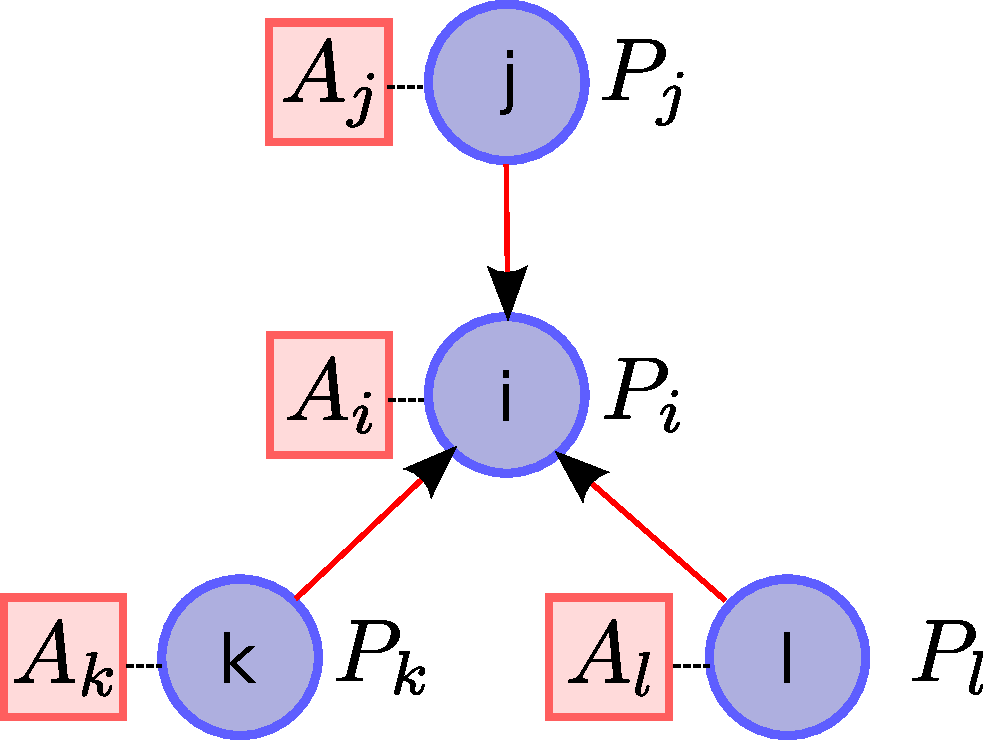
\includegraphics[width=.9\textwidth]{./Figures/gossip_2.pdf}
            \end{center}
            }
            \only<3>{
                \begin{center}
                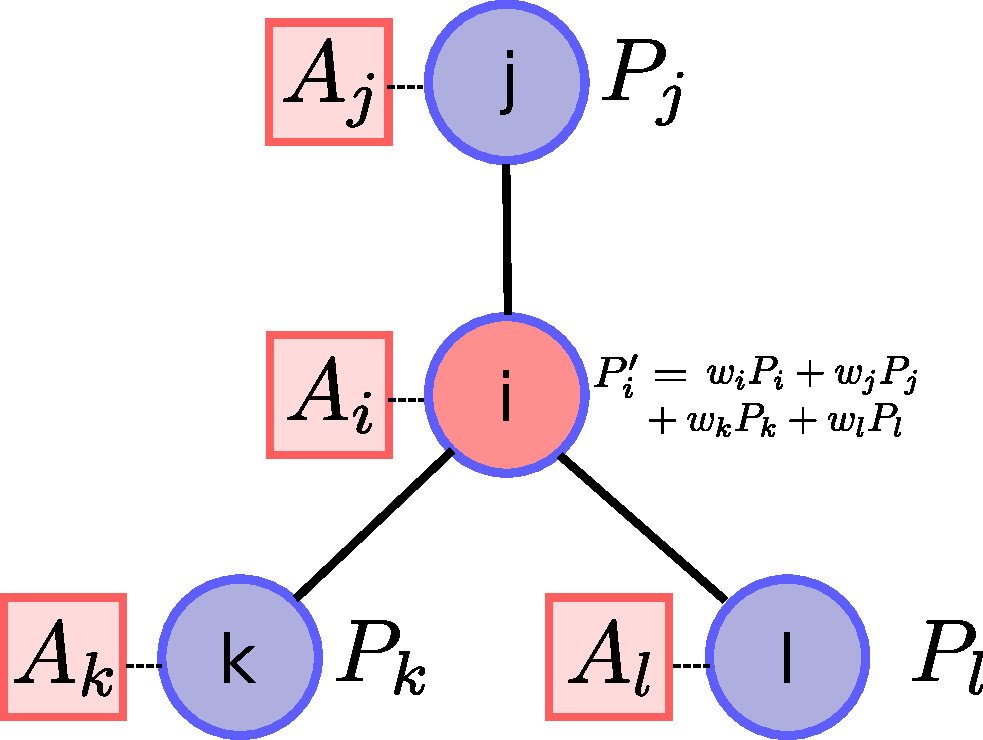
\includegraphics[width=.9\textwidth]{./Figures/gossip_3.pdf}
            \end{center}
            }
            \only<4>{
                \begin{center}
                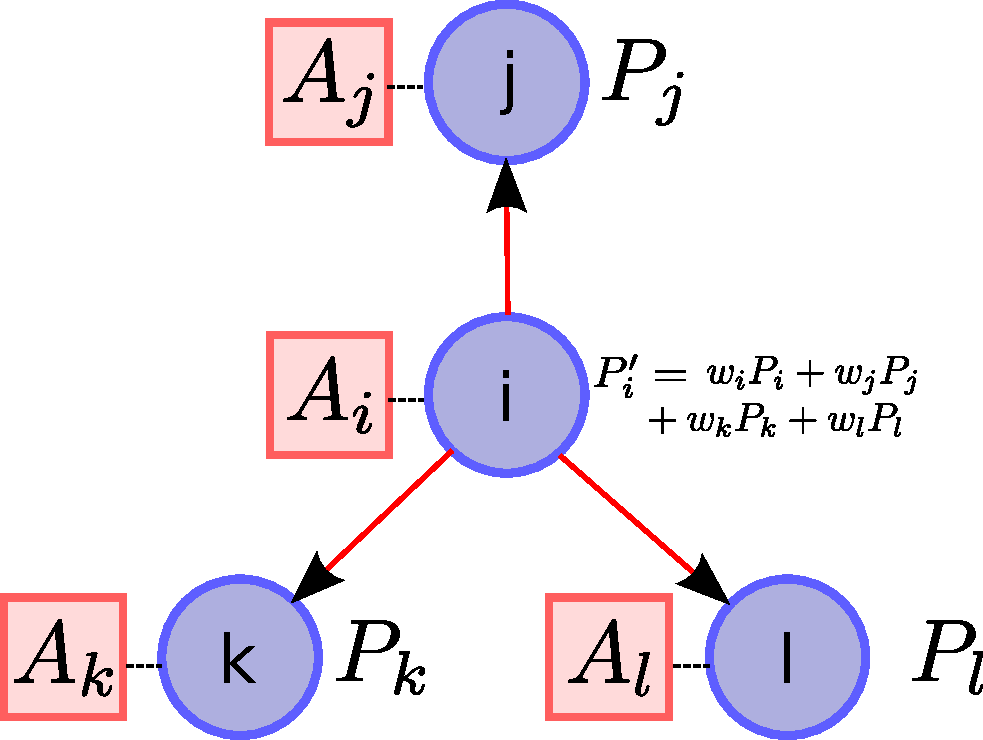
\includegraphics[width=.9\textwidth]{./Figures/gossip_4.pdf}
            \end{center}
            }
            \only<5,6>{
                \begin{center}
                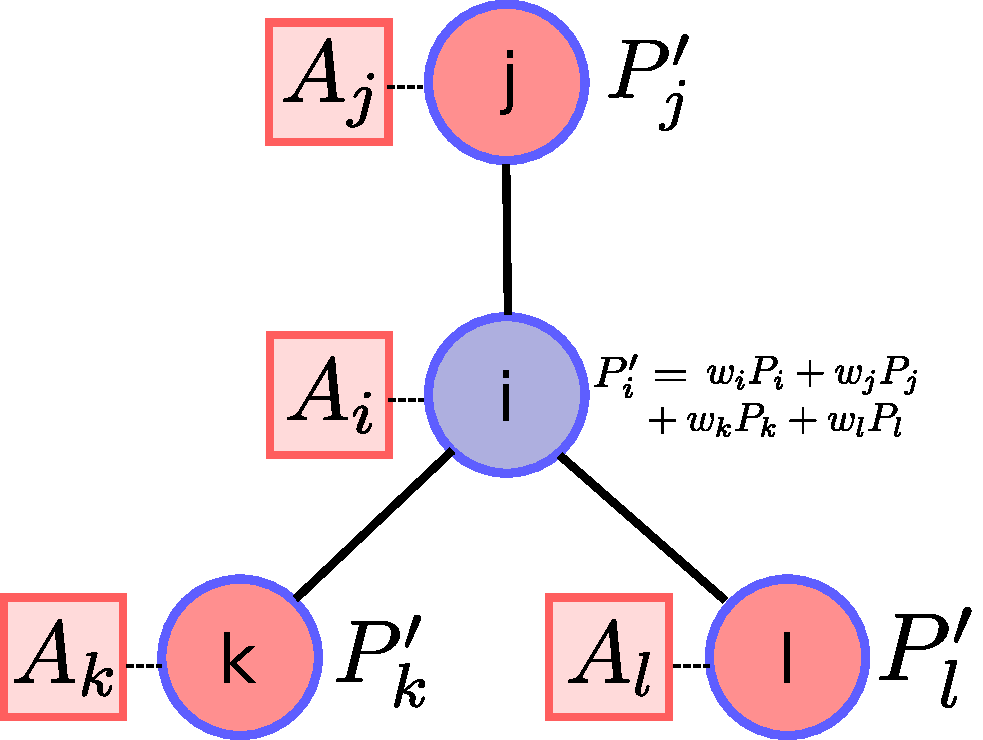
\includegraphics[width=.9\textwidth]{./Figures/gossip_5.pdf}
            \end{center}
            }
        \end{column}
    \end{columns}

    \vspace{.5cm}
    \onslide<6->{
    Nombreuses variantes possibles :
    \begin{itemize}
        \item Transmission de l'information
            \begin{itemize}
                \item synchrone/asynchrone
                \item stochastique/totale
            \end{itemize}
        \item Limitation du volume de donn\'ees transmises
        \item Graphe dynamique
        \item Donn\'ees dynamiques
    \end{itemize}
}
\end{frame}

\begin{frame}
    \frametitle{Exemple : K-means}

        K-means :
    \begin{itemize}
        \item explications k-means
    \end{itemize}
\end{frame}

\begin{frame}
    \frametitle{K-means par \emph{gossip}}

\end{frame}

\section{Estimation de la dissimilarit\'e}
\begin{frame}
    \frametitle{Estimation}

    \begin{itemize}
        \item Pour $P \in \mathcal{P}$, on aimerait calculer :
        \[
            w(P) = \frac{1}{n^2} \sum_{1 \leq i,j \leq n} D(X_i, X_j) \Phi_P(X_i, X_j)
        \]
        \item Problème : certains $D(X_i, X_j)$ inaccessibles
        \item Id\'ee : estimer $f : x \mapsto \mathbb{E}\left[ D(x, X) \Phi_P(x, X) \right]$

    \end{itemize}
\end{frame}

\end{document}


